%!TEX root = emnlp2016.tex

Foreign embassies of the United States government communicate with
each other and with the U.S. State Department through cabled message.
The National Archive collects these documents in a running corpus,
which traces the (unclassified) diplomatic history of the United
States. It has collected, for example, about two
million cables sent between 1973 and 1978.

Typically, a cable from this collection describes diplomatic ``business as usual,'' such as arrangements for visiting officials, recovery of lost or stolen passports, or obtaining lists of names for meetings and conferences. For example,
the embassies sent 8,635 cables during the week of April 21, 1975. Here is one,
selected at random,
\begin{shaded*} \tt{Hoffman, UNESCO Secretariat, requested info from
PermDel concerning an official invitation from the USG
RE subject meeting scheduled 10-13 JUNE 1975, Madison,
Wisconsin.  Would appreciate info RE status of action to 
be taken in order to inform Secretariat.  Hoffman communicating 
with Dr.~John P.~Klus RE list of persons to be invited.}
\end{shaded*}

But hidden in the corpus are also cables about important diplomatic
events, the cables and events that are of primary interest to
historians. During that same week, the United States was in the last
moments of the Vietnam war and, on April 30, 1975, lost its hold on Saigon. This resulted in the end of the Vietnam War and a max exodus of refugees from the country.  One
of the cables around this event is
\begin{shaded*}
  \tt{GOA program to move Vietnamese Refugees to Australia
  is making little progress and probably will not cover more than
  100-200 persons.  Press comment on smallness of program has
  recognized difficulty of getting Vietnamese out of Saigon, but
  ``Canberra Times'' Apr 25 sharply critical of government's
  performance.  [...]
  %Opposition continues to attack smallness of program,
  %but seems concerned, as does government, with scoring
  %point of domestic political importance.  With Parliament in
  %recess for next three weeks and Prime Minister on trip, issue
  %may attract less attention.
  Labor government clearly hopes whole
  matter will somehow disappear.}
\end{shaded*}

% cheating by putting this here...
\begin{figure*}[ht]
\centering
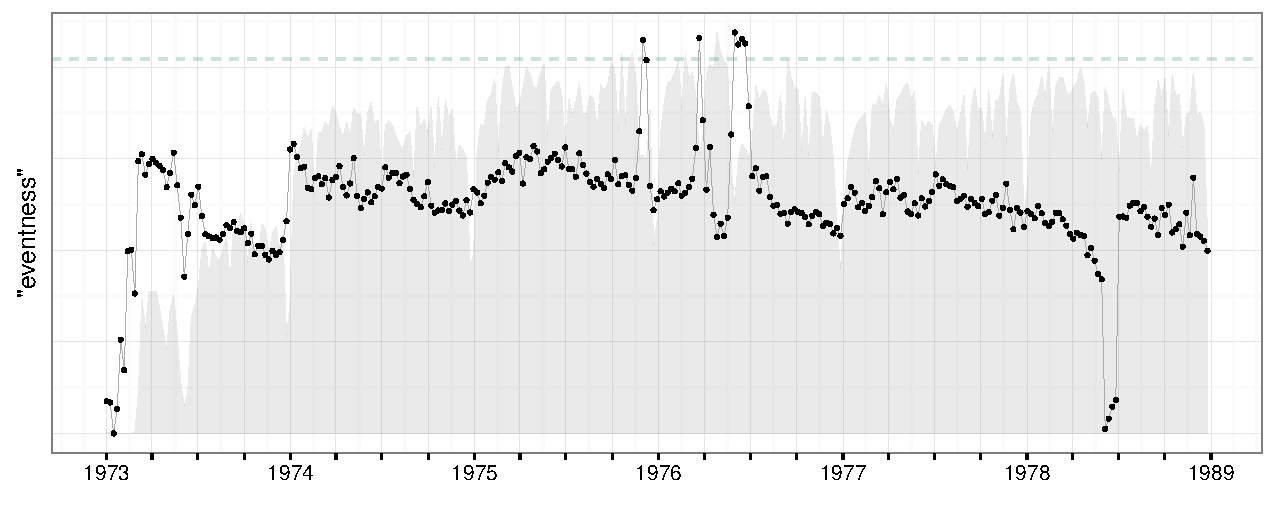
\includegraphics[width=\linewidth]{fig/cables_events.pdf}
\caption{Measure of ``eventness,'' or time interval impact on cable content (Eq.~\ref{eq:eventness}).  Grey background indicates the number of cables sent over time.  This comes from the model fit we discuss in \Cref{sec:eval}.  Capsule successful detects real-world events from National Archive diplomatic cables.}
\label{fig:cables_events}
\end{figure*}

Our goal in this paper is to develop a method to help historians and
political scientists wade through their collections, such as the 1970s
cables, to find potentially important events, such as the fall of
Saigon, and the primary sources around them. We develop
\textit{Capsule}, a probabilistic model for detecting and
characterizing important events in large collections of historical
communication.

\Cref{fig:cables_events} illustrates Capsule's analysis of the two
million cables from the National Archives. The \mbox{$y$-axis} is
``eventness'', a loose measure how strongly a week's cables deviate
from the usual diplomatic chatter to discuss a matter that is common
to many embassies. (This is described in detail in Section~\ref{sec:model}.)

The figure shows that Capsule detects many of the important moments
during this five-year span, including Indonesia's invasion of East
Timor (Dec. 7, 1975), the Air France hijacking and Israeli rescue operation
(June 27--July 4, 1976), and the fall of Saigon (April 30, 1975). It also identifies other moments,
such as the U.S. sharing lunar rocks with other countries (March 21, 1973) and
the death of Mao Tse-tung (Sept. 9, 1976). Broadly speaking, Capsule gives a
picture of the diplomatic history of these five years; it identifies
and characterizes moments and source material that might be of
interest to a historian.

The intuition behind Capsule is this: embassies write cables
throughout the year, usually describing typical business such as the
visiting of a government official. Sometimes, however, there is an
important event, e.g., the fall of Saigon. When an event occurs, it
pulls embassies away from their typical business to write cables that
discuss what happened and its consequences. Thus Capsule effectively
defines an ``event'' to be a moment in history when embassies deviate
from what each usually discusses, and when each embassy deviates in
the same way.

Capsule embeds this intuition into a Bayesian model. It uses hidden
variables to encode what ``typical business'' means for each embassy,
how to characterize the events of each week, and which cables discuss
those events. Given a corpus, the corresponding posterior distribution
provides a filter on the cables that isolates important moments in the
diplomatic history. \Cref{fig:cables_events} illustrates the mean of this
posterior.

Capsule can be used to explore any corpora with the same underlying
structure: text (or other discrete multivariate data) generated over time by known entities.  This includes
email, consumer behavior, social media posts, and opinion articles.

We present the model in Section~\ref{sec:model}, providing both a formal
model specification and guidance on how to use its posterior to detect 
and characterize real-worlds events.
In Section~\ref{sec:eval}, we evaluate Capsule and explore its results on
a collection of U.S. State Department cables and on simulated data.

\parhead{Related work.} We first review previous work on automatic
event detection and other related concepts.

% While Capsule uses text documents and associated metadata as input, event detection is often performed with univariate input data.  In this context, bursts that deviate from typical behavior (e.g., noisy constant or a repeating pattern) can define an event \cite{kleinberg2003bursty,ihler2007learning}; Poisson Processes~\cite{Kingman:1993} are often used to model events under this definition.  Alternatively, events can be construed as ``change points'' to mark when typical observations shift semi-permanently from one value to another~\cite{guralnik1999event}.
In both univariate and multivariate settings, the goal is often that analysts want to predict whether or not rare events will occur~\cite{weiss1998learning,das2008anomaly}.  Capsule, in contrast, is designed to help analysts explore and understand the original data: our goal is interpretability, not prediction.

Events can also be construed as ``change points'' to mark when typical observations shift semi-permanently from one value to another~\cite{guralnik1999event,adams2007bayesian}. Both varieties of events are important, but we focus on temporary shifts away from normal.

% Text is often used in event detection, as it is an abundant source of data.  
% In some applications, documents themselves are considered to be observed events~\cite{mccallum1998comparison,peng2007event}, or events are predetermined and tracked through the documents~\cite{yang2000improving,VanDam:2012}.  We are interested in detecting \emph{unobserved} events which can be characterized by patterns in the data.
%\newpage % note:when using hyperref, references can be split between pages!
A common goal is to identify clusters of documents; these approaches are used on news articles~\cite{zhao2012novel,zhao2007temporal,zhang2002novelty,li2005probabilistic,wang2007mining,allan1998line} and social media posts~\cite{VanDam:2012,lau2012line,jackoway2011identification,sakaki2010earthquake,reuter2012event,becker2010learning,sayyadi2009event}.  
In the case of news articles, the task is to create new clusters as novel news stories appear---this does not help disentangle typical content from rare events of interest.
Social media approaches identify rare events, but the methods are designed for short, noisy documents; they are not appropriate for larger documents that contain information about a variety of subjects.

Many existing methods use document terms as features, usually weighted by tf-idf value~\cite{fung2005parameter,kumaran2004text,brants2003system,das2011dynamic,zhao2007temporal,zhao2012novel}; here, events are bursts in groups of terms. % Because language is high dimensional, using terms as features limits scalability.

Topic models~\cite{Blei:2012} reduce the dimensionality of text data; they have been used to help detect events mentioned in social media posts~\cite{lau2012line,dou2012leadline} and posts relevant to monitored events~\cite{VanDam:2012}.
We rely on topic models to characterize both typical content and events, but grouped observations can also be summarized directly~\cite{peng2007event,chakrabarti2011event,gao2012joint}.

In addition to text data over time, author~\cite{zhao2007temporal}, news outlet~\cite{wang2007mining}, and spatial information~\cite{Neill:2005,mathioudakis2010identifying,liu2011using} can be used to augment event detection.  Capsule uses author information in order to characterize the typical concerns of authors.

Detecting and characterizing relationships~\cite{schein2015bayesian,linderman2014discovering,das2011dynamic} is related to event detection.  When a message recipient is known, Capsule can use a sender-receiver pair in place of an author, but the model could be further tailored for network interactions.

% TODO: cite he2015hawkestopic
